
\documentclass[border={7pt 0pt 185pt 0pt},varwidth]{standalone}
\usepackage{amsmath}
\usepackage{tikz-cd,tikz-3dplot} 
\usepackage{quiver}
\usepackage{diagbox}
\usepackage{xcolor}%colors
\usepackage{makecell}
\usepackage{adjustbox}
\usepackage[width=0.5,tiewidth=0.7]{strands}
\usetikzlibrary{calc,intersections,through,backgrounds,decorations.pathmorphing, decorations.shapes,decorations.markings,patterns}
%include other needed packages here   

\DeclareMathOperator{\GL}{\operatorname{GL}}
\DeclareMathOperator{\SL}{\operatorname{SL}}
\DeclareMathOperator{\supp}{supp}
\DeclareMathOperator{\dist}{dist}
\DeclareMathOperator{\vol}{vol}
\DeclareMathOperator{\diag}{diag}
\DeclareMathOperator{\tr}{tr}
\DeclareMathOperator{\Img}{\operatorname{Im}}
\DeclareMathOperator{\Id}{\operatorname{Id}}
\DeclareMathOperator{\rep}{\operatorname{rep}}
\DeclareMathOperator{\Rep}{\operatorname{Rep}}
\DeclareMathOperator{\RRep}{\widetilde{\operatorname{Rep}}}
\DeclareMathOperator{\Mod}{\operatorname{Mod}}
\DeclareMathOperator{\Hom}{\operatorname{Hom}}
\DeclareMathOperator{\Ext}{\operatorname{Ext}}
\DeclareMathOperator{\gldim}{\operatorname{gl.dim}}
\DeclareMathOperator{\projdim}{\operatorname{proj.dim}}
\DeclareMathOperator{\injdim}{\operatorname{inj.dim}}
\DeclareMathOperator{\dimv}{\operatorname{\underline{\mathbf{dim}}}}
\DeclareMathOperator{\Pic}{\operatorname{Pic}}
\DeclareMathOperator{\Jac}{\operatorname{Jac}}
\DeclareMathOperator{\ptt}{\operatorname{par}}
\newcommand{\Spec}{\operatorname{Spec}}
\DeclareMathOperator{\St}{\mathcal{Z}}
\DeclareMathOperator{\Flagd}{\operatorname{Flag}_{\mathbf{d}}}
\DeclareMathOperator{\Flagdstr}{\operatorname{Flag}_{\mathbf{d},str}}
\newcommand{\Gr}{\operatorname{Gr}}
\newcommand{\Grr}{\operatorname{Gr}}
\newcommand{\Grq}{\operatorname{Gr}^{KQ}}
\newcommand{\Flag}[1]{\operatorname{Flag}_{\mathbf{#1}}}
\newcommand{\Flagstr}[1]{\operatorname{Flag}_{\mathbf{#1},str}}
\newcommand{\dimvec}[1]{\mathbf{#1}}
\newcommand{\abdimvec}[1]{|\dimvec{#1}|}
\newcommand{\ftdimvec}[1]{\underline{\dimvec{#1}}}
\newcommand{\absgp}[1]{\mathbb{#1}}
\newcommand{\ww}{\varpi}
\DeclareMathOperator{\MinWd}{\operatorname{Min}(\absgp{W}_{\abdimvec{d}},W_{\dimvec{d}})}
\DeclareMathOperator{\Compd}{\operatorname{Comp}_{\dimvec{d}}}
\DeclareMathOperator{\Shuffled}{\operatorname{Schuffle}_{\dimvec{d}}}
\newcommand{\WWd}{\absgp{W}_{\abdimvec{d}}}
\newcommand{\Wd}{W_{\dimvec{d}}}

\newcommand{\Omcell}{\Omega}
\newcommand{\OOmcell}{\boldsymbol{\Omega}}
\newcommand{\Vcell}{\mathcal{V}}
\newcommand{\VVcell}{\boldsymbol{\mathcal{V}}}
\newcommand{\Ocell}{\mathcal{O}}
\newcommand{\OOcell}{\boldsymbol{\mathcal{O}}}

%\newcommand{\lbox}{\adjustbox{cfbox=red, margin=-\fboxrule-\fboxsep}}
\newcommand{\lbox}{\adjustbox{}}

\newenvironment{smbmatrix}% environment name
{% begin code
\bgroup
\setlength\arraycolsep{1pt}
\renewcommand{\arraystretch}{0.6}
\setcellgapes{0.2ex}
  \begin{bmatrix}
}%
{\end{bmatrix}
\egroup
}% end code
\newenvironment{smpmatrix}% environment name
{% begin code
\bgroup
\setlength\arraycolsep{1pt}
\renewcommand{\arraystretch}{0.8}
\setcellgapes{0.2ex}
  \begin{pmatrix}
}%
{\end{pmatrix}
\egroup
}% end code
\begin{document}

\begin{table}[ht]
 \[\setcellgapes{0.8ex}\makegapedcells
 \begin{array}{|ccccc|c|cc|c|cc|ccc|}
  \hline
  \multicolumn{5}{|c|}{\ww=wu} &w&\multicolumn{2}{|c|}{\ftdimvec{d},u} &\text{order of basis}&l(\ww) & l(w) & \absgp{B}_{\ww} & B_{\ww} & \ww B \ww^{-1}\\
  \hline
 \Id & \Id & \begin{smpmatrix}
   1\,2\,3\\ 1\,2\,3
   \end{smpmatrix} & \lbox{\parbox[h][][c]{1cm}{ 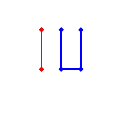
\begin{tikzpicture}[scale=0.5]
  \vpartition[
  floor=0,
  tkzpic=0,
  type=0
  ]{{3}}
  \tie[color=red,bull=1,bulletie=0.04,style=solid]{{1,1},{1,0}}
  \tie[color=blue,bull=1,bulletie=0.04,style=solid]{{2,1},{2,0}}
  \tie[color=blue,bull=1,bulletie=0.04,style=solid]{{3,1},{3,0}}
  \tie[color=blue,bull=1,bulletie=0.04,style=solid,tieheight=0]{{2},{3}}
  \end{tikzpicture}}} &\hspace{-2mm} \begin{smbmatrix}
   \scriptstyle 1&&\\
   &\scriptstyle 1&\\
   &&\scriptstyle 1\\
   \end{smbmatrix} & \lbox{\parbox[h][][c]{1cm}{\permutation[tkzpic=1,type=0,scale=0.5]{1,2,3}}} & abb & \lbox{\parbox[h][][c]{1cm}{ 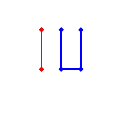
\begin{tikzpicture}[scale=0.5]
    \vpartition[
    floor=0,
    tkzpic=0,
    type=0
    ]{{3}}
    \tie[color=red,bull=1,bulletie=0.04,style=solid]{{1,1},{1,0}}
    \tie[color=blue,bull=1,bulletie=0.04,style=solid]{{2,1},{2,0}}
    \tie[color=blue,bull=1,bulletie=0.04,style=solid]{{3,1},{3,0}}
    \tie[color=blue,bull=1,bulletie=0.04,style=solid,tieheight=0]{{2},{3}}
    \end{tikzpicture}}} & \{v_1,v_2,v_3\} & 0 & 0 &  \begin{smbmatrix}
     *&*&*\\
     &*&*\\
     &&*\\
     \end{smbmatrix}& \begin{smbmatrix}
     *&&\\
     &*&*\\
     &&*\\
       \end{smbmatrix} & \begin{smbmatrix}
     *&&\\
     &*&*\\
     &&*\\
         \end{smbmatrix} \\ \hline
         

 t & (23) & \begin{smpmatrix}
   1\,2\,3\\ 1\,3\,2
   \end{smpmatrix} & \lbox{\parbox[h][][c]{1cm}{ 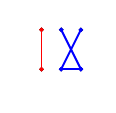
\begin{tikzpicture}[scale=0.5]
  \vpartition[
  floor=0,
  tkzpic=0,
  type=0
  ]{{3}}
  \tie[color=red,bull=1,bulletie=0.04,style=solid]{{1,1},{1,0}}
  \tie[color=blue,bull=1,bulletie=0.04,style=solid]{{3,1},{2,0}}
  \tie[color=blue,bull=1,bulletie=0.04,style=solid]{{2,1},{3,0}}
  \tie[color=blue,bull=1,bulletie=0.04,style=solid,tieheight=0]{{2},{3}}
  \end{tikzpicture}}} &\hspace{-2mm} \begin{smbmatrix}
   \scriptstyle 1&&\\
   &&\scriptstyle 1\\
   &\scriptstyle 1&\\
   \end{smbmatrix} & \lbox{\parbox[h][][c]{1cm}{\permutation[tkzpic=1,type=0,scale=0.5]{1,3,2}}} & abb & \lbox{\parbox[h][][c]{1cm}{ 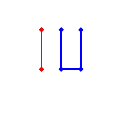
\begin{tikzpicture}[scale=0.5]
    \vpartition[
    floor=0,
    tkzpic=0,
    type=0
    ]{{3}}
    \tie[color=red,bull=1,bulletie=0.04,style=solid]{{1,1},{1,0}}
    \tie[color=blue,bull=1,bulletie=0.04,style=solid]{{2,1},{2,0}}
    \tie[color=blue,bull=1,bulletie=0.04,style=solid]{{3,1},{3,0}}
    \tie[color=blue,bull=1,bulletie=0.04,style=solid,tieheight=0]{{2},{3}}
    \end{tikzpicture}}} & \{v_1,v_3,v_2\} & 1 & 1 &  \begin{smbmatrix}
     *&*&*\\
     &*&\\
     &*&*\\
     \end{smbmatrix}& \begin{smbmatrix}
     *&&\\
     &*&\\
     &*&*\\
       \end{smbmatrix} & \begin{smbmatrix}
     *&&\\
     &*&\\
     &*&*\\
         \end{smbmatrix} \\ \hline
         
 s & (12) & \begin{smpmatrix}
   1\,2\,3\\ 2\,1\,3
   \end{smpmatrix} & \lbox{\parbox[h][][c]{1cm}{ 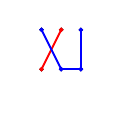
\begin{tikzpicture}[scale=0.5]
  \vpartition[
  floor=0,
  tkzpic=0,
  type=0
  ]{{3}}
  \tie[color=red,bull=1,bulletie=0.04,style=solid]{{2,1},{1,0}}
  \tie[color=blue,bull=1,bulletie=0.04,style=solid]{{1,1},{2,0}}
  \tie[color=blue,bull=1,bulletie=0.04,style=solid]{{3,1},{3,0}}
  \tie[color=blue,bull=1,bulletie=0.04,style=solid,tieheight=0]{{2},{3}}
  \end{tikzpicture}}} &\hspace{-2mm} \begin{smbmatrix}
   &\scriptstyle 1&\\
   \scriptstyle 1&&\\
   &&\scriptstyle 1\\
   \end{smbmatrix} & \lbox{\parbox[h][][c]{1cm}{\permutation[tkzpic=1,type=0,scale=0.5]{1,2,3}}} & bab & \lbox{\parbox[h][][c]{1cm}{ 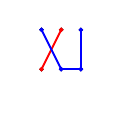
\begin{tikzpicture}[scale=0.5]
    \vpartition[
    floor=0,
    tkzpic=0,
    type=0
    ]{{3}}
    \tie[color=red,bull=1,bulletie=0.04,style=solid]{{2,1},{1,0}}
    \tie[color=blue,bull=1,bulletie=0.04,style=solid]{{1,1},{2,0}}
    \tie[color=blue,bull=1,bulletie=0.04,style=solid]{{3,1},{3,0}}
    \tie[color=blue,bull=1,bulletie=0.04,style=solid,tieheight=0]{{2},{3}}
    \end{tikzpicture}}} & \{v_2,v_1,v_3\} & 1 & 0 &  \begin{smbmatrix}
     *&&*\\
     *&*&*\\
     &&*\\
     \end{smbmatrix}& \begin{smbmatrix}
     *&&\\
     &*&*\\
     &&*\\
       \end{smbmatrix} & \begin{smbmatrix}
     *&&*\\
     &*&\\
     &&*\\
         \end{smbmatrix} \\ \hline
         
 ts & (132) & \begin{smpmatrix}
   1\,2\,3\\ 3\,1\,2
   \end{smpmatrix} & \lbox{\parbox[h][][c]{1cm}{ 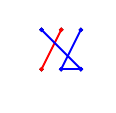
\begin{tikzpicture}[scale=0.5]
  \vpartition[
  floor=0,
  tkzpic=0,
  type=0
  ]{{3}}
  \tie[color=red,bull=1,bulletie=0.04,style=solid]{{2,1},{1,0}}
  \tie[color=blue,bull=1,bulletie=0.04,style=solid]{{3,1},{2,0}}
  \tie[color=blue,bull=1,bulletie=0.04,style=solid]{{1,1},{3,0}}
  \tie[color=blue,bull=1,bulletie=0.04,style=solid,tieheight=0]{{2},{3}}
  \end{tikzpicture}}} &\hspace{-2mm} \begin{smbmatrix}
   &\scriptstyle 1&\\
   &&\scriptstyle 1\\
   \scriptstyle 1&&\\
   \end{smbmatrix} & \lbox{\parbox[h][][c]{1cm}{\permutation[tkzpic=1,type=0,scale=0.5]{1,3,2}}} & bab & \lbox{\parbox[h][][c]{1cm}{ 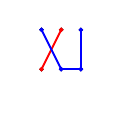
\begin{tikzpicture}[scale=0.5]
    \vpartition[
    floor=0,
    tkzpic=0,
    type=0
    ]{{3}}
    \tie[color=red,bull=1,bulletie=0.04,style=solid]{{2,1},{1,0}}
    \tie[color=blue,bull=1,bulletie=0.04,style=solid]{{1,1},{2,0}}
    \tie[color=blue,bull=1,bulletie=0.04,style=solid]{{3,1},{3,0}}
    \tie[color=blue,bull=1,bulletie=0.04,style=solid,tieheight=0]{{2},{3}}
    \end{tikzpicture}}} & \{v_3,v_1,v_2\} & 2 & 1 &  \begin{smbmatrix}
     *&*&\\
     &*&\\
     *&*&*\\
     \end{smbmatrix}& \begin{smbmatrix}
     *&&\\
     &*&\\
     &*&*\\
       \end{smbmatrix} & \begin{smbmatrix}
     *&*&\\
     &*&\\
     &&*\\
         \end{smbmatrix} \\ \hline
         
 st & (123) & \begin{smpmatrix}
   1\,2\,3\\ 2\,3\,1
   \end{smpmatrix} & \lbox{\parbox[h][][c]{1cm}{ 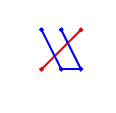
\begin{tikzpicture}[scale=0.5]
  \vpartition[
  floor=0,
  tkzpic=0,
  type=0
  ]{{3}}
  \tie[color=red,bull=1,bulletie=0.04,style=solid]{{3,1},{1,0}}
  \tie[color=blue,bull=1,bulletie=0.04,style=solid]{{1,1},{2,0}}
  \tie[color=blue,bull=1,bulletie=0.04,style=solid]{{2,1},{3,0}}
  \tie[color=blue,bull=1,bulletie=0.04,style=solid,tieheight=0]{{2},{3}}
  \end{tikzpicture}}} &\hspace{-2mm} \begin{smbmatrix}
   &&\scriptstyle 1\\
   \scriptstyle 1&&\\
   &\scriptstyle 1&\\
   \end{smbmatrix} & \lbox{\parbox[h][][c]{1cm}{\permutation[tkzpic=1,type=0,scale=0.5]{1,2,3}}} & bba & \lbox{\parbox[h][][c]{1cm}{ 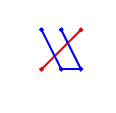
\begin{tikzpicture}[scale=0.5]
    \vpartition[
    floor=0,
    tkzpic=0,
    type=0
    ]{{3}}
    \tie[color=red,bull=1,bulletie=0.04,style=solid]{{3,1},{1,0}}
    \tie[color=blue,bull=1,bulletie=0.04,style=solid]{{1,1},{2,0}}
    \tie[color=blue,bull=1,bulletie=0.04,style=solid]{{2,1},{3,0}}
    \tie[color=blue,bull=1,bulletie=0.04,style=solid,tieheight=0]{{2},{3}}
    \end{tikzpicture}}} & \{v_2,v_3,v_1\} & 2 & 0 &  \begin{smbmatrix}
     *&&\\
     *&*&*\\
     *&&*\\
     \end{smbmatrix}& \begin{smbmatrix}
     *&&\\
     &*&*\\
     &&*\\
       \end{smbmatrix} & \begin{smbmatrix}
     *&&\\
     &*&\\
     *&&*\\
         \end{smbmatrix} \\ \hline
         
 sts & (13) & \begin{smpmatrix}
   1\,2\,3\\ 3\,2\,1
   \end{smpmatrix} & \lbox{\parbox[h][][c]{1cm}{ 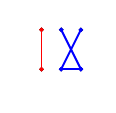
\begin{tikzpicture}[scale=0.5]
  \vpartition[
  floor=0,
  tkzpic=0,
  type=0
  ]{{3}}
  \tie[color=red,bull=1,bulletie=0.04,style=solid]{{1,1},{1,0}}
  \tie[color=blue,bull=1,bulletie=0.04,style=solid]{{3,1},{2,0}}
  \tie[color=blue,bull=1,bulletie=0.04,style=solid]{{2,1},{3,0}}
  \tie[color=blue,bull=1,bulletie=0.04,style=solid,tieheight=0]{{2},{3}}
  \end{tikzpicture}}} &\hspace{-2mm} \begin{smbmatrix}
   &&\scriptstyle 1\\
   &\scriptstyle 1&\\
   \scriptstyle 1&&\\
   \end{smbmatrix} & \lbox{\parbox[h][][c]{1cm}{\permutation[tkzpic=1,type=0,scale=0.5]{1,3,2}}} & bba & \lbox{\parbox[h][][c]{1cm}{ 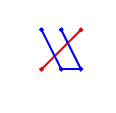
\begin{tikzpicture}[scale=0.5]
    \vpartition[
    floor=0,
    tkzpic=0,
    type=0
    ]{{3}}
    \tie[color=red,bull=1,bulletie=0.04,style=solid]{{3,1},{1,0}}
    \tie[color=blue,bull=1,bulletie=0.04,style=solid]{{1,1},{2,0}}
    \tie[color=blue,bull=1,bulletie=0.04,style=solid]{{2,1},{3,0}}
    \tie[color=blue,bull=1,bulletie=0.04,style=solid,tieheight=0]{{2},{3}}
    \end{tikzpicture}}} & \{v_3,v_2,v_1\} & 3 & 1 &  \begin{smbmatrix}
     *&&\\
     *&*&\\
     *&*&*\\
     \end{smbmatrix}& \begin{smbmatrix}
     *&&\\
     &*&\\
     &*&*\\
       \end{smbmatrix} & \begin{smbmatrix}
     *&&\\
     *&*&\\
     &&*\\
         \end{smbmatrix} \\ \hline
 \end{array}
 \]
        
\end{table}
\end{document}